\documentclass[11pt,a4paper]{article}
\usepackage[T1]{fontenc}
\usepackage{lmodern,amsmath,amssymb,booktabs,microtype,graphicx}
\usepackage[margin=24mm]{geometry}
\usepackage[colorlinks=true,urlcolor=blue,linkcolor=blue]{hyperref}
\newcommand{\Js}{\mathcal J_s}
\newcommand{\C}{\mathcal C}
\DeclareMathOperator{\sech}{sech}
\title{The derivative singlet at first order\\Fixed-time connected four-point dynamics}
\author{Alan Day \and Chengheng\thanks{AI research assistant (OpenAI).}}
\date{Local research note --- 6 November 2026}
\begin{document}\maketitle
\begin{abstract}
We apply established semiclassical chord four-point functions to a
derivative singlet of complex DSSYK after removing its conserved part. Keeping all three
same-species pairings gives an explicit connected kernel at arbitrary fixed
real times, and closed first-order expressions for the commutator squared
and the adjacent-time cumulant. Exact chord moments and a finite-deformation
four-arc implementation provide independent checks. This supplies a
microscopic interaction target for the Susskind Rindler-meson program.
\end{abstract}

\section{Observable, state, and result}
We use the full annealed normalized trace $\tau$ at $\beta=\mu=0$, standard
CAR, and units $\hbar=c_{\rm light}=1$. In the normalization of the preceding
local singlet notes,
\begin{align}
 A&=\sum_i[H,c_i]^\dagger[H,c_i],& O&=A-\mathbb E A(Q),\notag\\
 B&=H^2-\mathbb E H^2(Q),&X&=(O-cB)/\sqrt{W_d},\notag\\
 c&=2\lambda\frac{1-q}{1+q},&
 W_d&=4\Js^4\left[\lambda^{-1}+\frac{4q}{1+q}\right].
\end{align}
Here $Q$ is fermion number. The Hermitian Gaussian ensemble is
$H=\sum_{|I|=|J|=p}G_{IJ}c_I^\dagger c_J$, including overlaps, with
\[
 \mathbb E G_{IJ}G_{KL}=w\delta_{IL}\delta_{JK},\qquad
 w=4^p\frac{\Js^2}{\lambda}\left(\frac{p!}{N^p}\right)^2.
\]
First take $N,p\to\infty$ at $p^2/N=\lambda>0$; then expand at small
$\lambda$ with fixed string times. Our previous mixed-chord reduction has
$Q_{HH}=q$, $Q_{HX}=q^2$, $Q_{XX}=q^4$. Set
\begin{equation}
 h=4\lambda,\quad q=e^{-h},\quad H_{\rm src}=H/(2\Js),\quad
 u_j=2\Js t_j,\quad d=2,\quad \tau(H_{\rm src}^2)=1/h.
\end{equation}
Write $g_{ij}=\sech^{2d}(u_i-u_j)$ and $T_{ij}=\tanh(u_i-u_j)$.
The cumulant subtracts the \emph{full finite-$h$} two-point functions:
\begin{equation}
 \kappa_4=\tau(X_1X_2X_3X_4)
 -G_{12,h}G_{34,h}-G_{23,h}G_{41,h}-G_{13,h}G_{24,h}.
\end{equation}
The resulting fixed-time semiclassical coefficient is
\begin{align}
 \kappa_4&=hK_4+O(h^2),\notag\\
 K_4&=-d^2\left[g_{12}g_{34}T_{12}T_{34}
 +g_{23}g_{41}T_{23}T_{41}\right.\notag\\
 &\hspace{23mm}\left.
 +g_{13}g_{24}\frac{\cosh(u_1+u_3-u_2-u_4)}
 {\cosh(u_1-u_3)\cosh(u_2-u_4)}\right].\label{general}
\end{align}
The formula uses the sourced expansion in Refs.~\cite{lin,streicher}; the
remainder notation is asymptotic, not a certified uniform numerical bound.

\newpage
\section{Two useful closed functions}
Define $X(t)=e^{iHt}Xe^{-iHt}$ and the positive tracial observable
\begin{equation}
 \C(t)=\tau\bigl([X(t),X]^\dagger[X(t),X]\bigr)
 =2\{F_{22}(t)-F_{\rm OTO}(t)\},
\end{equation}
where $F_{22}=\tau(X(t)^2X^2)$ and
$F_{\rm OTO}=\tau(X(t)XX(t)X)$. At both orderings the disconnected
part is $1+2G_h(t)^2$. It cancels exactly before any expansion.
With $u=2\Js t$, Eq.~\eqref{general} gives
\begin{align}
 K_{22}(u)&=d^2(2\tanh^2u-1)\sech^{4d}u,\label{adj}\\
 K_{\rm OTO}(u)&=-d^2\left[\cosh(2u)
 +2\tanh^2u\,\sech^{4d}u\right],\\
 \C(t)&=2hd^2\left[\cosh(2u)
 +(4\tanh^2u-1)\sech^{4d}u\right]+O(h^2).
\end{align}
For our $d=2$ singlet these become
\begin{align}
 \boxed{\C(t)=32\lambda\left[\cosh(4\Js t)
 +(4\tanh^2(2\Js t)-1)\sech^8(2\Js t)\right]+O(\lambda^2),}\label{comm}\\[3mm]
 \kappa_{22}(t)=16\lambda(2\tanh^2(2\Js t)-1)
 \sech^8(2\Js t)+O(\lambda^2).\label{kap}
\end{align}
The box in Eq.~\eqref{comm} concerns the model coefficient, with the limits
and normalization specified above. It is not an on-shell bulk coupling.

At short times, the coefficient reproduces
\begin{equation}
 \C(t)=1280\Js^2\lambda t^2+O(\lambda t^4\Js^4)+O(\lambda^2),\qquad
 \kappa_{22}(0)=-16\lambda+O(\lambda^2).
\end{equation}
Also $\kappa_{22}''(0)=768\Js^2\lambda+O(\lambda^2)$.
The leading adjacent cumulant changes sign at
\[\Js t=\tfrac12\operatorname{artanh}(1/\sqrt2)=0.4406868\ldots.\]
This is a zero of the coefficient, not an assertion about the exact
finite-$\lambda$ zero. The first-order commutator coefficient is positive
for $t\ne0$: if $\tanh^2u\ge1/4$ both terms in brackets are nonnegative;
otherwise their sum exceeds $1-\sech^8u>0$.

For $1\ll\Js t$ within a small-correction overlap window,
Eq.~\eqref{comm} has leading behavior $16\lambda e^{4\Js t}$.
This matches the earlier scrambling expansion. Taking times of order
$\log(1/\lambda)/(4\Js)$ requires the resummed kernel; the fixed-time
expansion alone does not justify that limit.

\section{What cancels and what must remain}
An expansion of $G_{q^2}$ or $G_{q^4}$ has its own first-order correction.
Those terms must be included if one computes $F_{22}$ in isolation.
Working with connected channels removes them algebraically. It does
\emph{not} remove either of the uncrossed channels. Retaining only the
crossed contribution would fail the adjacent cumulant and the early-time
commutator checks.

\newpage
\section{Source map and oriented insertions}
The tools are the two-sided OPE of Lin--Stanford, including their
Eq.~(205) and Appendix G, and Streicher's time-ordered and OTO correlators
\cite{lin,streicher}. Their chord deformation parameter is our $h=4\lambda$.
Streicher's interaction-order symbol $q$ is not our chord weight $q=e^{-h}$.

For the crossed pairing $(13)(24)$, continuation of Lin--Stanford's
two-sided variables at zero microscopic inverse temperature gives
\begin{equation}
 \tau_+=i(u_3-u_1),\quad \tau_+'=i(u_4-u_2),\quad
 \tau_-=i(u_1+u_3-u_2-u_4),\quad c_{\rm LS}\to1.
\end{equation}
The surviving normalized connected term in their (205) is
$-hd^2\cos(\tau_-)/[\cos(\tau_+)\cos(\tau_+')]$.
Multiplication by $g_{13}g_{24}$ produces the last term of
Eq.~\eqref{general}. At coincident times it equals $-hd^2$.
The mutual crossing factor $q^{d^2}$ is already represented in this
connected result; multiplying it a second time would double count.

For an uncrossed pairing, Appendix G.2 identifies leading energy exchange.
At zero inverse temperature the two-energy measure is invariant under
exchange of its arguments and simultaneous sign reversal. Thus, with
$s=u_i-u_j$ and the indicated operator order,
\begin{equation}
 \tau(H_{\rm src}X(u_i)X(u_j))
 =-\frac{i}{2}\partial_sG_h(s)
 =id\tanh(s)\sech^{2d}s+O(h).
\end{equation}
Dividing the product of two such matrix elements by
$\tau(H_{\rm src}^2)=1/h$ yields the first term of
Eq.~\eqref{general}. Cyclic rotation yields the second, with
\emph{oriented} separation $u_4-u_1$. Replacing $T_{41}$ by $T_{14}$
would reverse that contribution. In Appendix G.1 one must take the
zero-inverse-temperature limit after forming the products: a vanishing
variance prefactor multiplies divergent tangent coefficients.

\section{An exact finite-$q$ computational representation}
We generalize the previous BINT transfer implementation \cite{bint}
to four independent real times. In $\Js=1$ units let
\begin{equation}
 J_{n,n+1}=\lambda^{-1/2}\sqrt{\frac{1-q^{n+1}}{1-q}},\quad
 D_r=\operatorname{diag}(r^n),\quad r=q^2,\quad\chi=q^4,
\end{equation}
and set $a=(t_4-t_3,t_3-t_2,t_2-t_1,t_1-t_4)$,
$U_j=e^{ia_jJ}$. The two uncrossed contractions are
\begin{equation}
 A_0=(D_rU_3|0\rangle)^T U_2U_4(D_rU_1|0\rangle),\qquad
 A_1=\text{one cyclic shift of the four arc labels}.
\end{equation}
The transpose is bilinear, without complex conjugation. This distinction
also matters for the general crossed contraction on the next page.

\newpage
Put $f_n=(q;q)_n$, $b_i=(r^2;q)_i r^i/f_i$, and define the source matrix
\begin{equation}
 V^{(j)}_{li}=\sqrt{b_i}\,r^l\sqrt{f_{l+i}/f_l}\,(U_j)_{l+i,0}.
\end{equation}
The remaining channel and full function are
\begin{equation}
 R=\sum_{n,i}r^n(U_3V^{(4)})_{ni}(U_2V^{(1)})_{ni},\qquad
 F=A_0+A_1+\chi R.\label{bilinear}
\end{equation}
Only for the alternating ordering does $R$ reduce to the previous
positive Hilbert--Schmidt norm. General real times require the bilinear
product in Eq.~\eqref{bilinear}.

\section{Evidence and measured finite-deformation errors}
Exact integer chord polynomials, expanded with rational arithmetic in
$q=e^{-h}$, independently match 22 Taylor coefficients of
Eq.~\eqref{general}. The checks include 72 cancellations of nonpositive
Laurent powers. The time rays $(1,0,1,0)$ and $(1,1,0,0)$ extend through
$u^{10}$; $(2,1,-1,0)$ and $(0,1,3,-1)$ extend through $u^8$.
For example,
\begin{equation}
 \frac{\C}{h}=80u^2-\frac{640}{3}u^4+\frac{4352}{9}u^6
 -\frac{50888}{63}u^8+\frac{3150752}{2835}u^{10}+O(u^{12}).
\end{equation}
These checks constrain the closed formula locally, rather than proving
its remainder for arbitrary time.

A second implementation evaluates the original nonsymmetric BINT index
sum at 50 decimal digits, at the same finite size $L=14$. All 12 channel
comparisons at two deformations and two nonalternating time sets agree
with the symmetric implementation to absolute tolerance $10^{-12}$.
For the main computation, $\lambda=(.04,.02,.01,.005)$ uses respectively
$L=(169,332,672,1383)$. Selected $L+16$ channel changes are at most
$1.23\times10^{-15}$. Alternating reduction, cyclicity, reversal and common
time translation also pass. These are numerical representation and
stability checks, not a bound on all floating-point error.

\begin{center}
\begin{tabular}{rrrr}
\toprule
$\Js t$ & predicted $\C/h$ & extrapolated $\C/h$ & relative difference\\
\midrule
0.10 & 2.887655 & 2.869919 & $-0.61\%$\\
0.20 & 8.887575 & 8.819786 & $-0.76\%$\\
0.35 & 17.805892 & 17.465716 & $-1.91\%$\\
0.50 & 30.426106 & 28.771611 & $-5.44\%$\\
\bottomrule
\end{tabular}
\end{center}
Here extrapolation means $2(\C/h)_{\lambda=.005}-(\C/h)_{\lambda=.01}$;
it is not an error certificate. At $\Js t=.5$, the raw $\lambda=.005$
coefficient is $24.850065$, or $18.33\%$ below the leading prediction.
The corresponding extrapolated adjacent coefficient is $0.01986431$
against $0.01991637$, a $0.26\%$ difference.

The previous alternating-kernel cutoff parameters were reused
conservatively. Cauchy--Schwarz bounds a general bilinear contraction by
the product of its two Hilbert--Schmidt norms, but we have not completed a
new total cutoff proof for every arc here. The saved alternating cutoff
bound is therefore not a certified general-time error bar; selected
refinements provide the empirical control stated above.

\newpage
\begin{figure}[ht]
\centering
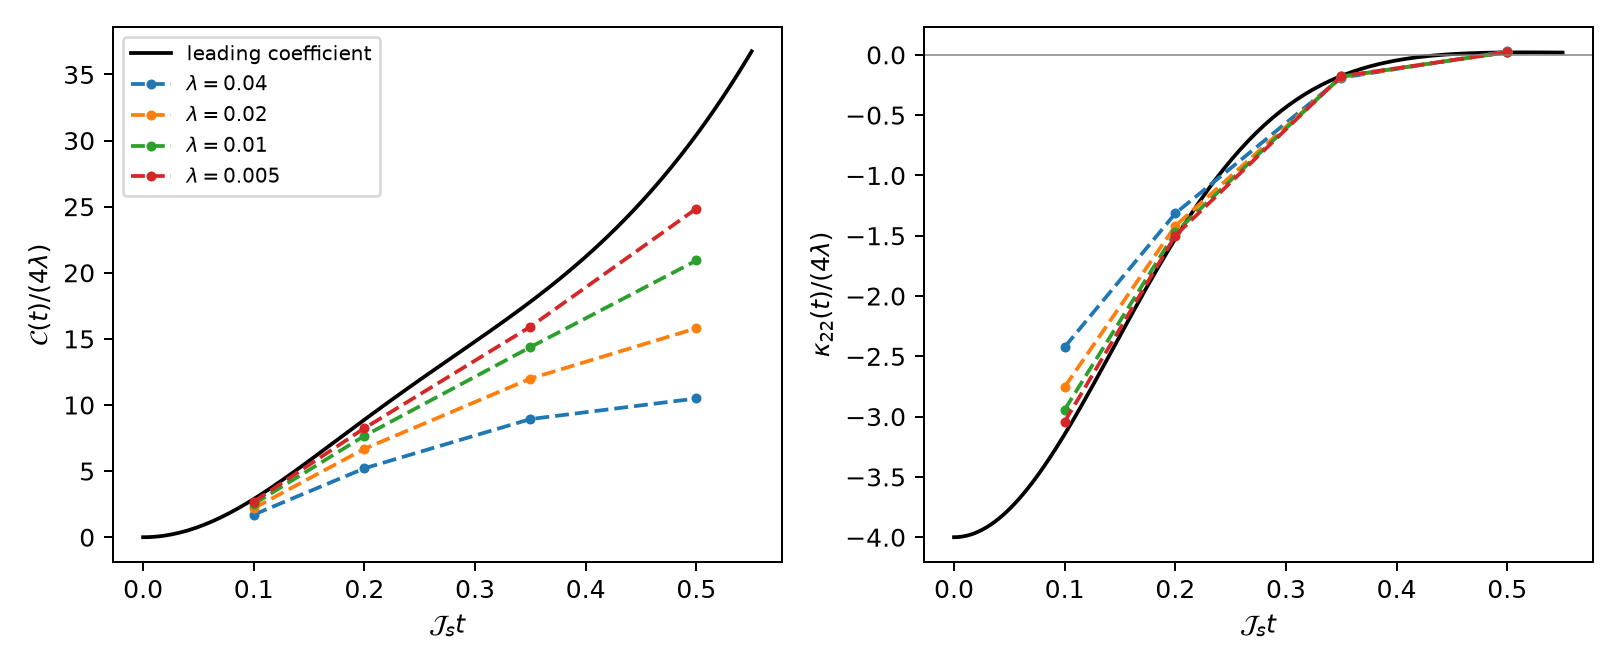
\includegraphics[width=\linewidth]{../../results/susskind-first-order/fixed-time-first-order.png}
\caption{Finite-$\lambda$ kernels compared with their first-order coefficients.
The commutator curve approaches its limit more slowly at the later times.}
\end{figure}
For the three nonalternating physical time sets
\[(.3,.1,-.1,0),\qquad(.2,-.05,.35,.1),\qquad(.15,.15,-.15,-.15),\]
the errors in
$\kappa_4/h$ at $\lambda=.005$ are respectively
$-0.0038913$, $+0.2446429$, $-0.0014850$.
All shrink from $.01$ to $.005$; the third is not monotone over the
entire four-deformation scan. Maximum observed crossed-sum cancellation
is $2.20$, and connected-subtraction condition number is $373$.
Absolute and coefficient errors are retained in the machine-readable data.

\section{The next physical construction}
The earlier regulated KG packet matched the singlet's midpoint two-point
function, with arbitrary positive mass absorbed in radial dilation.
Its ordinary equal-thermal-gap four-point value $33$ at zero real time
does not equal the microscopic value $3$. The present calculation fixes
the \emph{microscopic} three-channel multi-insertion target, using the
pair-dependent continuation underlying the fake-circle construction.
It has not yet supplied a spatial KG operator map preserving multiplication.

The next task is to construct an independent spatial or translation
observable and its cross-correlators with $X$. We will first examine the
chord generators and multiparticle representation, then test whether a
Rindler translation algebra and a mass observable survive the specified
limit. The chord label $d=2$ alone does not determine a Poincare mass.
This moves the project from temporal kernel matching toward the meson
spectrum and physical scattering dictionary.

\begin{thebibliography}{9}
\bibitem{lin} H. W. Lin and D. Stanford, \emph{A symmetry algebra in
double-scaled SYK}, \href{https://arxiv.org/abs/2307.15725}{arXiv:2307.15725}.
\bibitem{streicher} A. Streicher, \emph{SYK Correlators for All Energies},
\href{https://arxiv.org/abs/1911.10171}{arXiv:1911.10171}.
\bibitem{bint} M. Berkooz, M. Isachenkov, V. Narovlansky and G. Torrents,
\emph{Towards a full solution of the large $N$ double-scaled SYK model},
\href{https://arxiv.org/abs/1811.02584}{arXiv:1811.02584}.
\end{thebibliography}
\end{document}
